% !TeX root = ..\rapport_13_1.tex
\section{Kravspecifikation}
\subsection{Indledning}
\subsection{Ordliste}
\begin{table}[H]
    \centering
    \begin{tblr}{width = \textwidth, rowsep = 3px, colspec = {Q[l, font = \bfseries, wd = .17\textwidth]Q[l, wd = .73\textwidth]}}
        Medarbejder       & En medarbejder er en person ansat i Softwarehuset A/S, som er tildelt aktiviteter. En medarbejder kan udføre aktiviteter og registrere arbejdstid brugt på aktiviteter, uagtet om medarbejderen er tilknyttet aktiviteten. Hver medarbejder har et medarbejder ID. \\
        Projekt aktivitet & En delopgave af et projekt. Hver aktivitet er tilknyttet en medarbejder.                                                                                                                                                                                           \\
        Faste aktiviteter & Aktiviteter der ikke kan pålægges et projekt. F.eks. ferie, sygdom, kurser.                                                                                                                                                                                        \\
        Projekt           & Udviklingsarbejde udført for en kunde (eksternt) eller for Softwarehuset A/S (internt). Et projekt administreres af en projektleder og er inddelt i aktiviteter. Hvert projekt har et projektnummer.                                                               \\
        Kunde             & En ekstern entitet som bestiller og er modtager af projekter.                                                                                                                                                                                                      \\
        Projektleder      & En medarbejder der har ret til at oprette og tildele aktiviteter for et givent projekt.                                                                                                                                                                            \\
        Softwarehuset A/S & Entitet som er modtager af et projekt, hvis projektet er internt.                                                                                                                                                                                                  \\
        Medarbejder ID    & Identifikation for hver enkelt medarbejder. Består af fire bogstaver. To første fra fornavn efterfulgt af to første fra efternavn. F.eks. rawi.                                                                                                                    \\
        Projektnumer      & Identifikation for hvert enkelt projekt. Har formen årstal efterfulgt af et fireciffret løbenummer. F.eks. 23001                                                                                                                                                   \\
        Budgetteret tid   & En aktivitets fastlagte antal hele timer.                                                                                                                                                                                                                          \\
        Arbejdstid        & Mængde tid i inkrementer af halve timer, brugt på en aktivitet. Kan registreres af den medarbejder som har brugt arbejdstid på en given aktivitet.                                                                                                                 \\
    \end{tblr}
\end{table}
\subsection{Use case diagrammer}
\begin{figure}[H]
    \centering
    \caption{Use case diagram for programmet \textbf{Timeregistrering og projektstyring} hvori de tre aktører inkluderet er Gæst, Medarbejder og Projektleder.}\label{fig:AlleActorsPaaEnGang}
    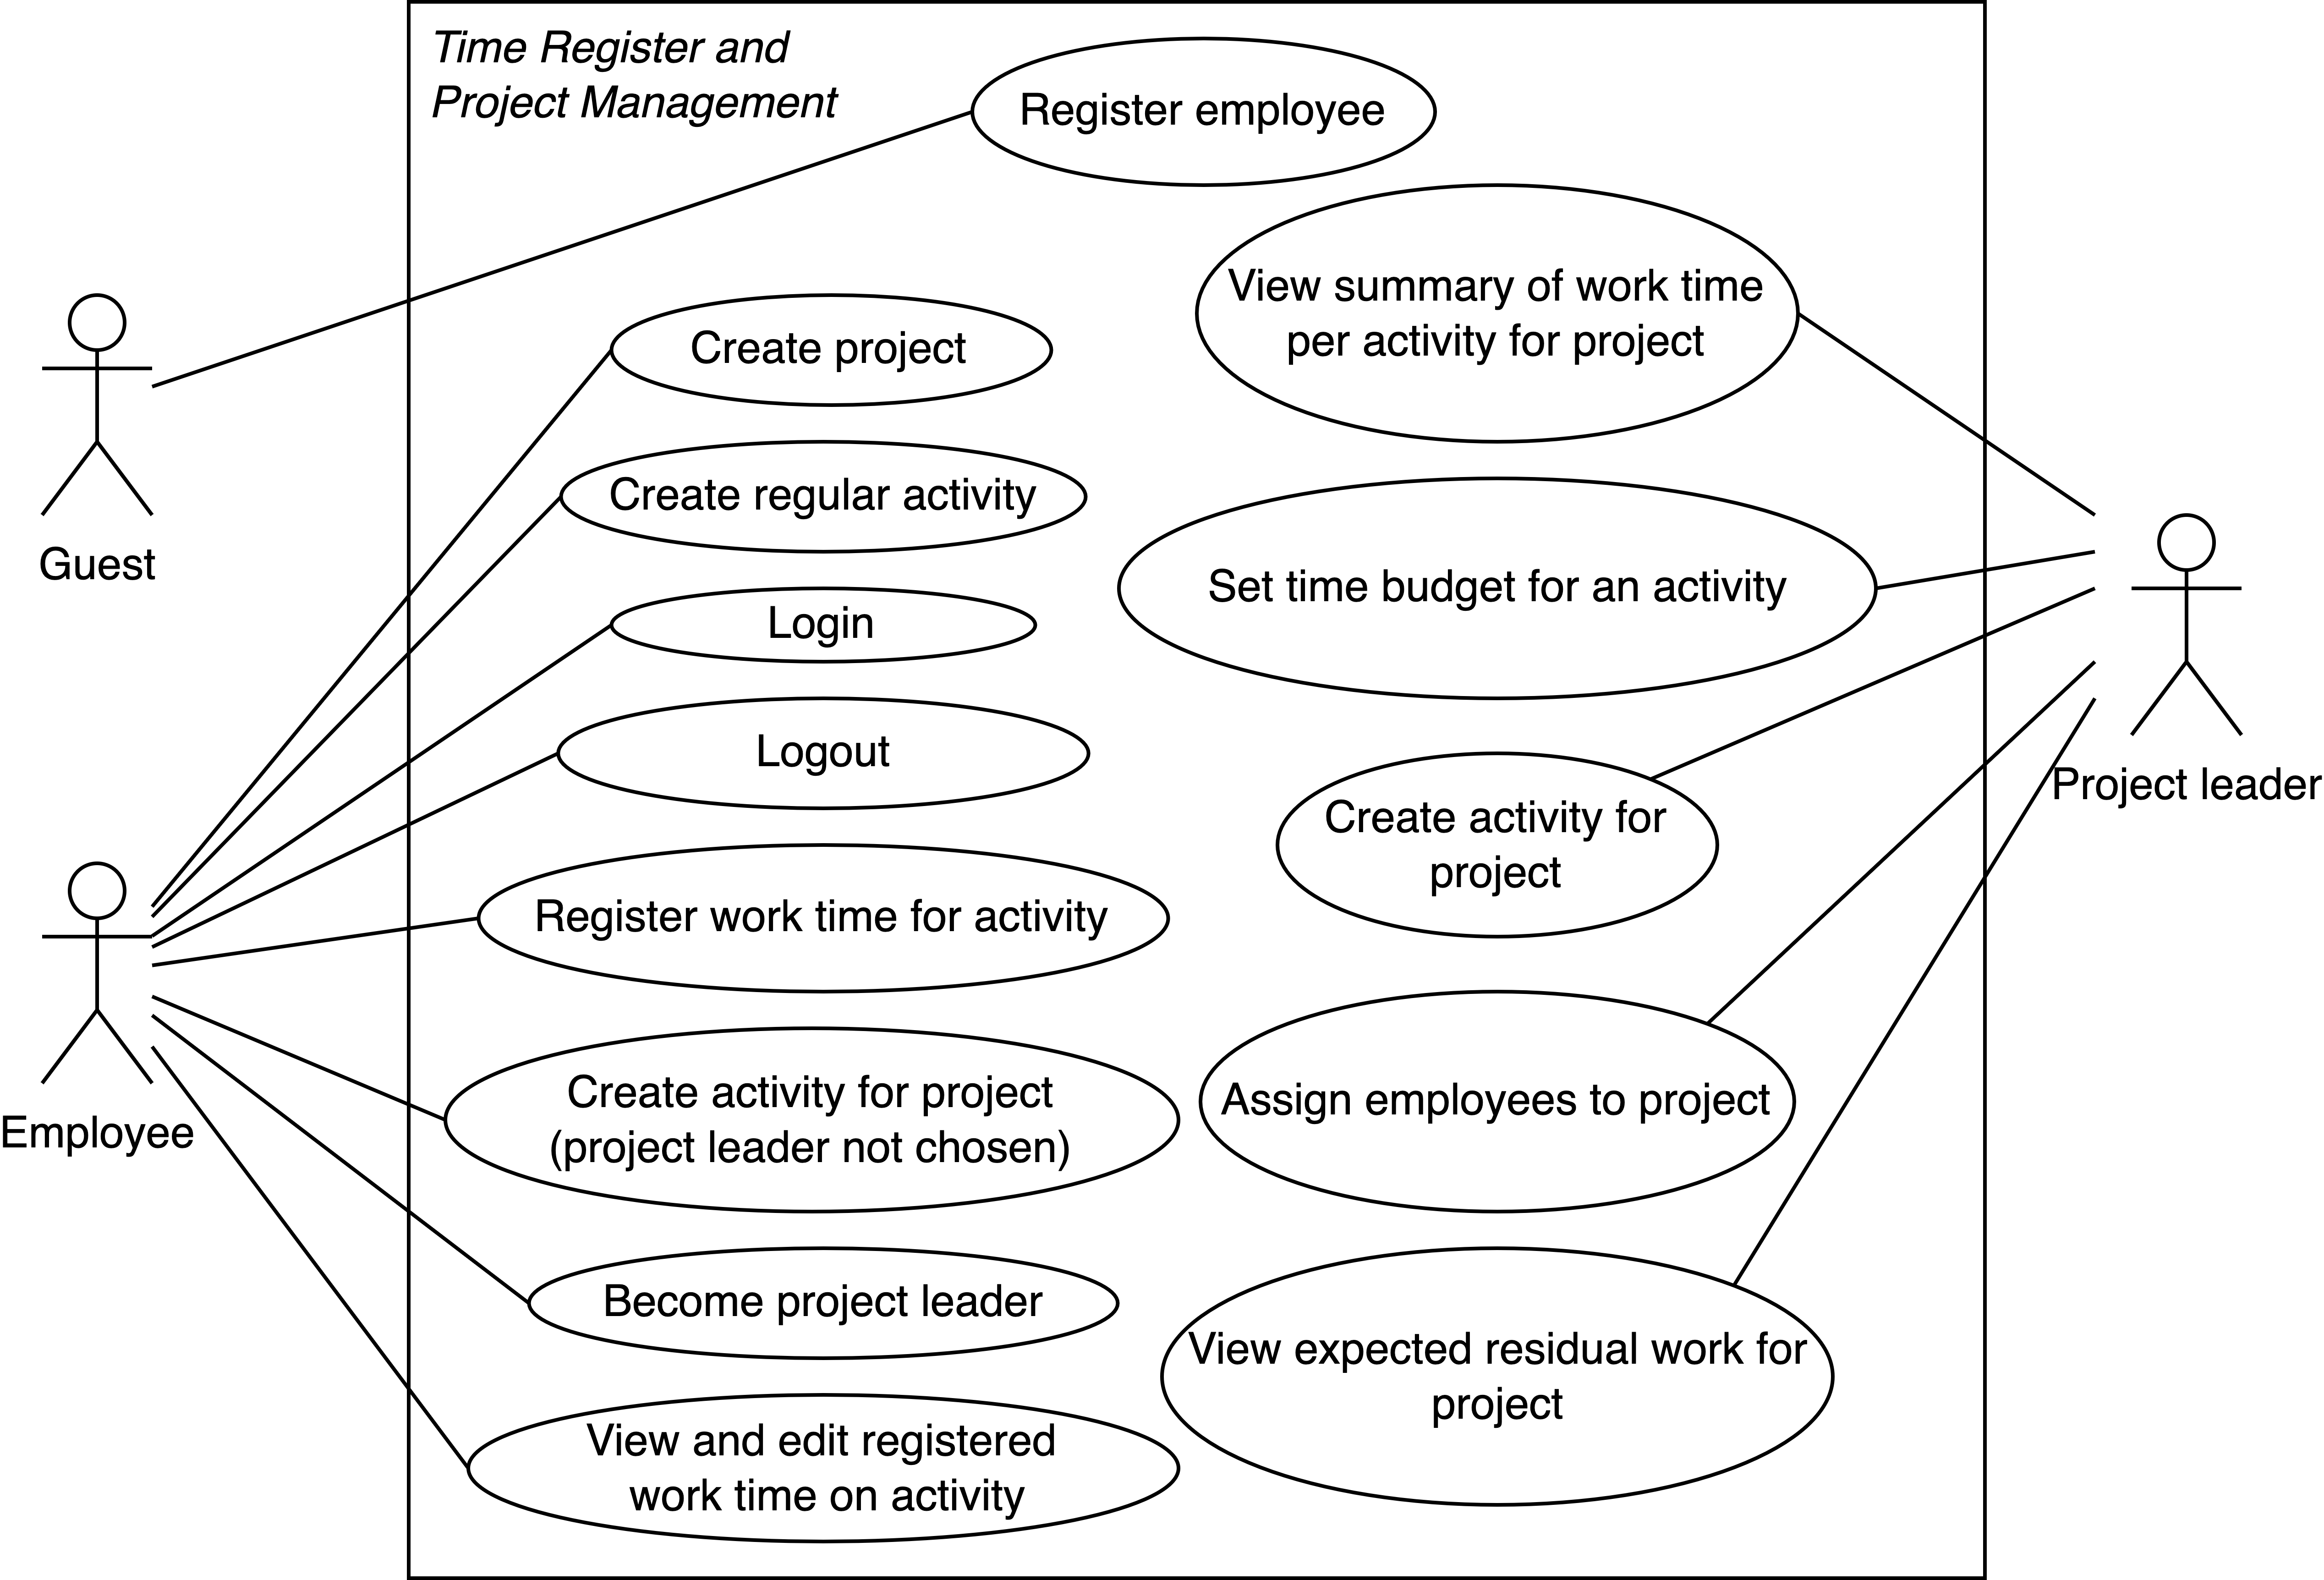
\includegraphics[width=.85\textwidth]{Diagrams/Timeregistrering og projektstyring.png}
\end{figure}
\begin{table}[H]
    \centering
    \caption{Todo usecases}
    \begin{tabular}{ll}
        Use case                                             & Tildelt \\
        \midrule
        Opret Medarbejder                                    &         \\
        Opret projekt                                        &         \\
        Opret fast aktivitet                                 &         \\
        Login                                                &         \\
        Registrer arbejdstid på aktivitet                    &         \\
        Opret Aktivitet for projekt (Medarbejder)            & Max     \\
        Påtag projektleder stilling                          & Max     \\
        Se og rediger i registreret arbejdstid på aktivitet  & Mathies \\
        Se oversigt over arbejdstid pr. aktivitet og projekt & Mathies \\
        Anfør budgetteret tid til løsning af aktivitet       &         \\
        Opret Aktivitet for projekt (Projektleder)           &         \\
        Tilknyt medarbejdere til projekt                     &         \\
        Se forventet restarbejde på projekt                  &         \\
    \end{tabular}
\end{table}

\subsection{Detaljerede use cases}
\begin{listing}[H]
    \centering
    \caption{Cucumber feature 1}\label{lst:feature1}
    \begin{minted}{gherkin}
    Feature: Buy fruit
    Description: A user buys fruit...
    Actors: User
        
    Scenario: Buy a fruit with enough money
        Given the vending machine has fruits
        When the user enters enough mone for a fruit
        And the user selects a fruit
        And the machine returns the rest money
        And the vending machine remembers its earnings
        ...
    \end{minted}
\end{listing}

\begin{listing}[H]
    \centering
    \caption{Cucumber feature 2}\label{lst:feature2}
    \begin{minted}{gherkin}
    Feature: Buy fruit
    Description: A user buys fruit...
    Actors: User
    
    Scenario: Buy a fruit with enough money
        Given the vending machine has fruits
        When the user enters enough mone for a fruit
        And the user selects a fruit
        And the machine returns the rest money
        And the vending machine remembers its earnings
        ...
    \end{minted}
\end{listing}

\subsection{Diskussion: Kravspecifikation}